
\documentclass[landscape,paperheight=24in,paperwidth=36in,fontscale=0.40]{baposter} % Adjust the font scale/size here
% original fontsize 0.44 
\title{HTML Cheat Sheet New}
\usepackage[brazilian]{babel}
\usepackage[utf8]{inputenc}

\usepackage{graphicx} % Required for including images
\graphicspath{{figures/}} % Directory in which figures are stored

\usepackage{xcolor}
\usepackage{colortbl}
\usepackage{tabu}

\usepackage{comment}

\usepackage{mathtools}
%\usepackage{amsmath} % For typesetting math
\usepackage{amssymb} % Adds new symbols to be used in math mode

\usepackage{booktabs} % Top and bottom rules for tables
\usepackage{enumitem} % Used to reduce itemize/enumerate spacing
\usepackage{palatino} % Use the Palatino font
\usepackage[font=small,labelfont=bf]{caption} % Required for specifying captions to tables and figures

\usepackage{multicol} % Required for multiple columns
\setlength{\columnsep}{1.5em} % Slightly increase the space between columns
\setlength{\columnseprule}{0mm} % No horizontal rule between columns

\usepackage{tikz} % Required for flow chart
\usetikzlibrary{decorations.pathmorphing}
\usetikzlibrary{shapes,arrows} % Tikz libraries required for the flow chart in the template

\newcommand{\compresslist}{ % Define a command to reduce spacing within itemize/enumerate environments, this is used right after \begin{itemize} or \begin{enumerate}
\newcommand{\legendre}[2]{\left(\frac{#1}{#2}\right)} % Define a command to show Legendre symbol modulo p
\setlength{\itemsep}{1pt}
\setlength{\parskip}{0pt}
\setlength{\parsep}{0pt}
}
\definecolor{orange}{RGB}{220,80,30}% Defines the color used for content box headers
 %\definecolor{lightblue}{rgb}{0.145,0.6666,1} 

\begin{document}

\begin{poster}
{
columns=2,
headerborder=closed, % Adds a border around the header of content boxes
colspacing=0.8em, % Column spacing
bgColorOne=white, % Background color for the gradient on the left side of the poster
bgColorTwo=white, % Background color for the gradient on the right side of the poster
borderColor=orange, % Border color
headerColorOne=black, % Background color for the header in the content boxes (left side)
headerColorTwo=orange, % Background color for the header in the content boxes (right side)
headerFontColor=white, % Text color for the header text in the content boxes
boxColorOne=white, % Background color of the content boxes
textborder=roundedleft, % Format of the border around content boxes, can be: none, bars, coils, triangles, rectangle, rounded, roundedsmall, roundedright or faded
eyecatcher=true, % Set to false for ignoring the left logo in the title and move the title left
headerheight=0.1\textheight, % Height of the header
headershape=roundedright, % Specify the rounded corner in the content box headers, can be: rectangle, small-rounded, roundedright, roundedleft or rounded
headerfont=\Large\bf\textsc, % Large, bold and sans serif font in the headers of content boxes
%textfont={\setlength{\parindent}{1.5em}}, % Uncomment for paragraph indentation
linewidth=2pt % Width of the border lines around content boxes
}
{\includegraphics[height=4em]{igl-logo-small.png}}
{\vspace{-1.2em} 
\bf\textsc{Interactive Visualizations with Mathematica
}}% Poster title
{\vspace{2.1em}
\large\bf\textsc{Scholars: Xiaojun Jia, Adithya Swaminathan,
	Dimitrios Tambakos, Troy Yang, Sarah Zimmerman
\\  Faculty Mentor: A.J. Hildebrand
\\  Project Leader: Efstathios Konstantinos Chrontsios Garitsis
\\ \vspace{0.05em} \normalsize{University of Illinois at Urbana-Champaign}}}
{\includegraphics[height=4em]{imark.png}}

%---------------------------------------------
% Project Goals
%---------------------------------------------
\headerbox{Julia Sets}{name=define,column=0,span=1}{
\begin{multicols}{3}
\begin{itemize}
    \item Let $P: \mathbb{C}\rightarrow\mathbb{C}$ be a polynomial and denote $P^{k}$ as the \mbox{k-th} iterate, 
    i.e. $$P^k=P\circ P \circ \dots P\quad \text{($k$ times)}$$ 
    \item We define the Julia set of $P$ to be the boundary of all the points $z \in \mathbb{C}$ for which the set $\{P^{k}(z) : k \in \mathbb{N}\}$ is bounded.
    \vfill
     \columnbreak
     \item The complement of the Julia set is the Fatou set.
     \item We are specifically \mbox{interested} in the nature of the Julia Set graph of cubic polynomials of the form ${z^3+re^{ti}z^2+e^{2 \pi i \theta}z}$ as the variables vary over $$r>0, t\in \mathbb{R}, \theta \in \mathbb{R}\setminus\mathbb{Q}$$
   
\end{itemize}
\columnbreak
\colorbox[HTML]{FFCBBF}{\makebox[0.3\textwidth-2\fboxsep][l]{\bf \large $r = 2$, $\theta = e^{\phi}$, $t = .70371$}}
\begin{center}
    \includegraphics[width=1.75in,height=1.5in]{jsetforposter.png}
\end{center}
\end{multicols}
\vspace*{-4ex}
}


\headerbox{Patterns in Julia Set Graphs
}{name=intro,column=0,span=1,below=define}{

%\begin{multicols}{1}
\colorbox[HTML]{FFCBBF}{\makebox[\textwidth-2\fboxsep][l]{\bf \large  Example Of A Pattern ($r = 4$, $\theta = \pi$, $t \in [0, 2\pi]$)}}
\\
\newline
As $r$ grows larger, we notice a specific pattern more often. Namely, when we change the value of $t$, the graphs rotate around (0,0) by angle $t$.

%\begin{center}
\begin{center}
\colorbox[HTML]{FFCBBF}{\makebox[\textwidth-2\fboxsep][l]{\bf \large \hspace{0.5in} $t=0$ \hspace{1.25in} $t=\pi/6$ \hspace{1.05in} $t=\pi/3$ \hspace{1.1in} $t=\pi/2$}}
\end{center}
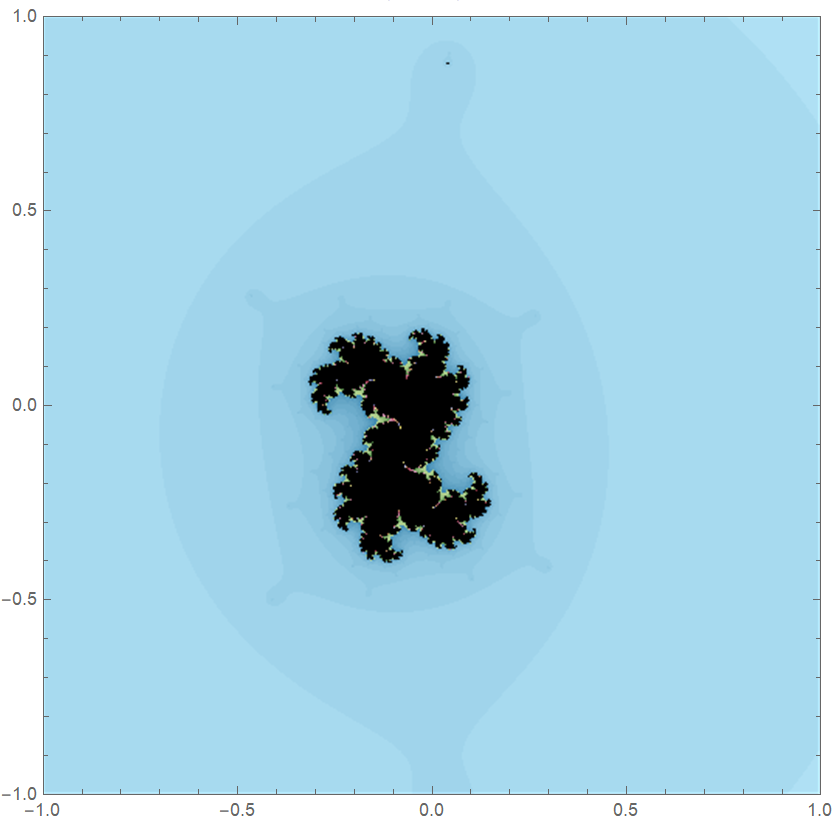
\includegraphics[width=1.5in,height=1.25in]{1.PNG}
\hspace{0.2in} 
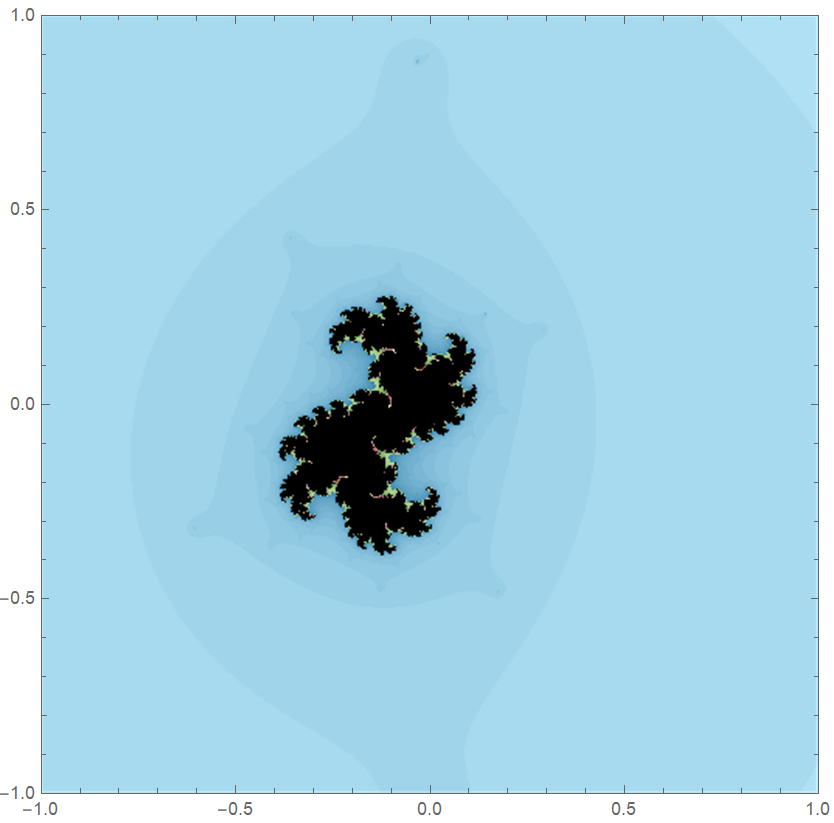
\includegraphics[width=1.5in,height=1.25in]{2.PNG}
%\end{center}
%\columnbreak
~
%\begin{center}
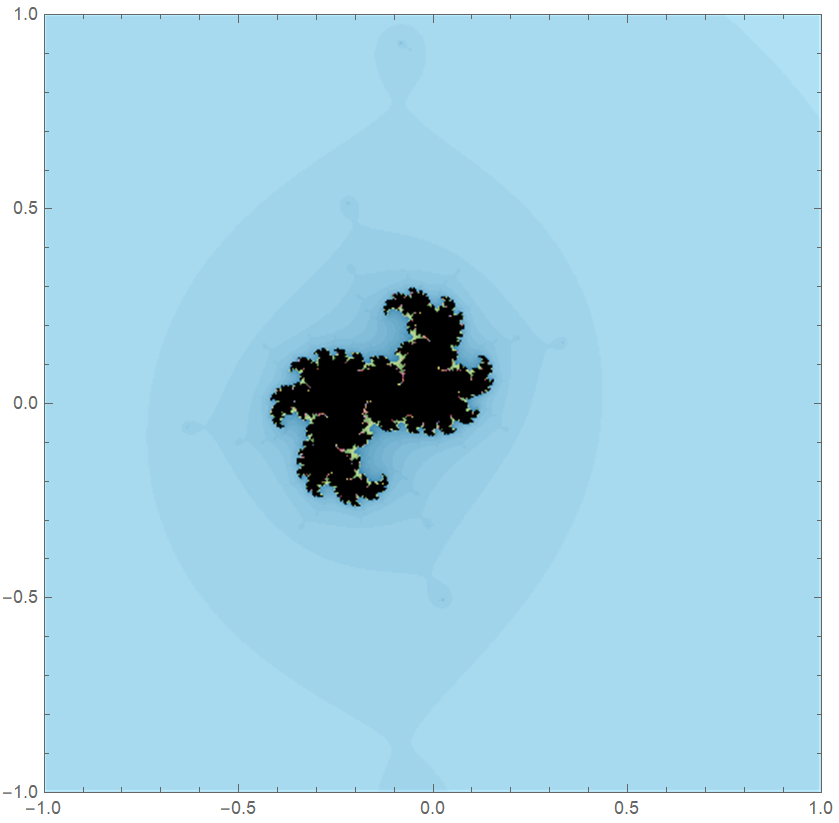
\includegraphics[width=1.5in,height=1.25in]{3.PNG} 
\hspace{0.15in} 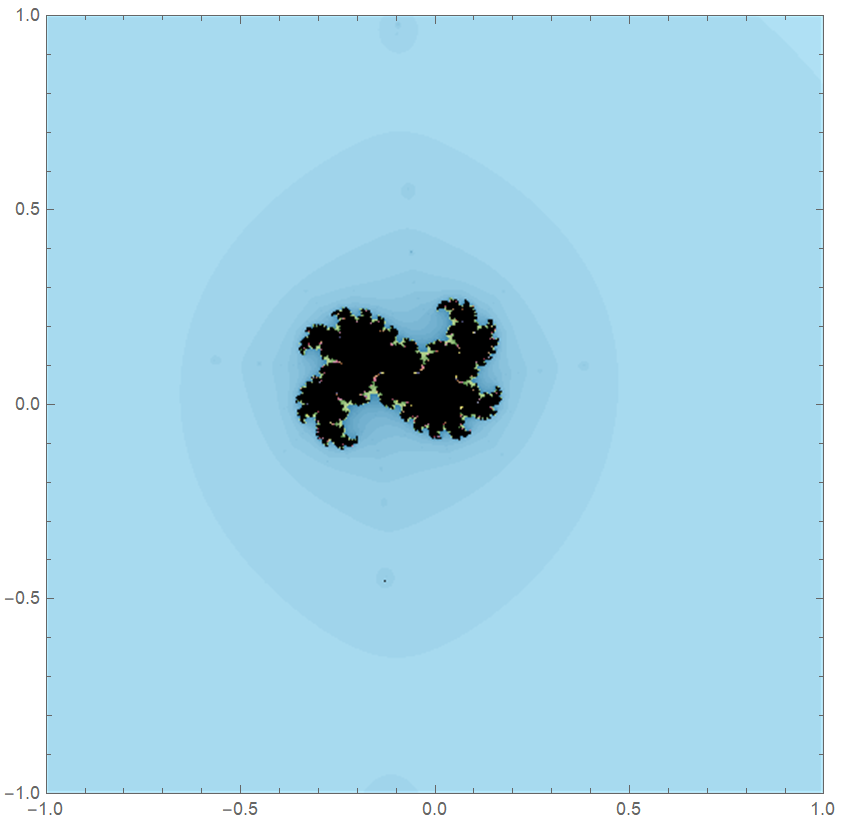
\includegraphics[width=1.5in,height=1.25in]{4.PNG}
%\end{center}
%\end{multicols}

\colorbox[HTML]{FFCBBF}{\makebox[\textwidth-2\fboxsep][l]{\bf \large Exceptions To The Discovered Pattern}}

\begin{multicols}{2}
However, the central symmetry pattern does not \mbox{appear} to hold for most $r$ closer to 1. \\

For example, take the graphs of the Julia Set of the \mbox{cubic} polynomial when $r=1.612$ and $t=-1.196$ and $t=1.196$, shown on the right respectively. It is clear that as the angle $t$ changes, the symmetric pattern does not hold.
\columnbreak
\begin{center}
\colorbox[HTML]{FFCBBF}{\makebox[0.45\textwidth-2\fboxsep][c]{\bf \large $z^3+1.612e^{\pm 1.196 i}z^2+e^{2\pi^{\pi+1}i}z$}}

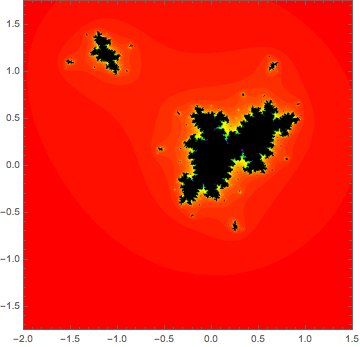
\includegraphics[width=0.45\linewidth]{pi2pi1.png}
\hspace{1em}
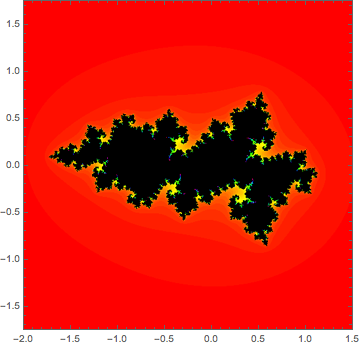
\includegraphics[width=0.45\linewidth]{pi2pi2.png}
\end{center}
\end{multicols}
}


\headerbox{References}{column=0,span=1,below=intro}{
\begin{itemize}[leftmargin=0.15in]\compresslist
\item Beardon, A. F., "Iteration of Rational Functions: Complex Analytic Dynamical Systems", \textit{Springer}, 1991.
\item Carleson, L., and Theodore W. Gamelin, "Complex Dynamics", \textit{Springer}, 1993.
\end{itemize}
}


\headerbox{Sum-Of-Digit Fractals}{name=fractals,column=1,span=1}{

\begin{multicols}{2}
\colorbox[HTML]{FFCBBF}{\makebox[0.48\textwidth-2\fboxsep][l]{\bf \large Definition}}
Let $b$ be an integer base, and let $p$ and $q$ be  some positive real parameters. The \textbf{sum-of-digit fractal} corresponding to base $b$, and parameters $p$ and $q$ is the graph 
with steps given by 
\[e ^ {2 \pi i (s_b(n)/p + n/q)},
\quad n=1,2,3,\dots, \]
where $s_b(n)$ is the sum-of-digit function and $q$ and $p$ are parameters. 

\vspace{1ex}

    
\newline

Observe that the $n$-th step has unit length and direction given by the angle $2 \pi  (s_b(n)/p + n/q)$.
\columnbreak
\vspace{-4.8ex}
%\begin{itemize}
\colorbox[HTML]{FFCBBF}{\makebox[0.48\textwidth-2\fboxsep][l]{\bf \large Theorem (Lehmer \& Lehmer, 1979)}}
\begin{itemize}
\item If $b \equiv 1 \pmod{p}$, and $q = 1$, the fractal is finite and represents a regular $p$-gon.
\item If $b \equiv 0 \pmod{p}$, and $q = 1$, the fractal is finite and consists of $p$ rotations of a regular $p$-gon about a fixed point.
\end{itemize}
The most interesting cases are the ones where at least one of $p$ and $q$ is irrational (Dekking, 1982; Dekking \& Mendes-France, 1981). In those cases, the fractals obtained are infinite. The following slides illustrate these cases.
\end{multicols}
\vspace{-0.9ex}
}




\headerbox{Examples of Sum-of-Digit Fractals
}{name=fractalexamples,column=1,span=1,below=fractals}{
\begin{multicols}{2}
\colorbox[HTML]{FFCBBF}{\makebox[0.48\textwidth-2\fboxsep][l]{\bf \large $N = 3000$, $b = 3$, $p = 5$, $q = 3$}}
    \begin{center}
    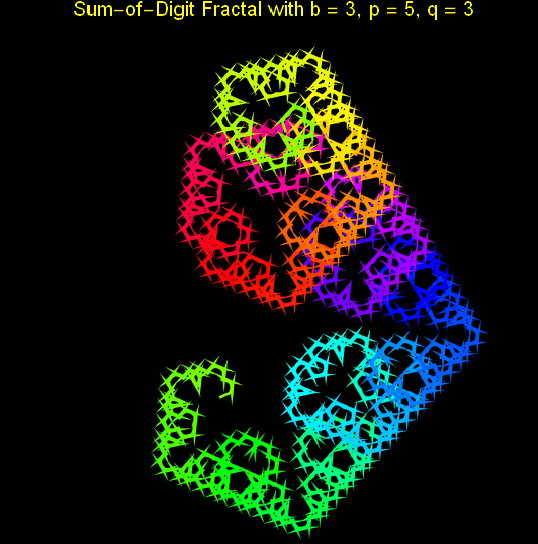
\includegraphics[width=0.48\textwidth,
    height=0.45\textwidth]{n3000v2.png}
    \end{center}
    \vfill
\columnbreak
\colorbox[HTML]{FFCBBF}{\makebox[0.48\textwidth-2\fboxsep][l]{\bf \large $N = 10 000$, $b = 2$, $p = 3$, $q = \ln(2)$}}
    \begin{center}
    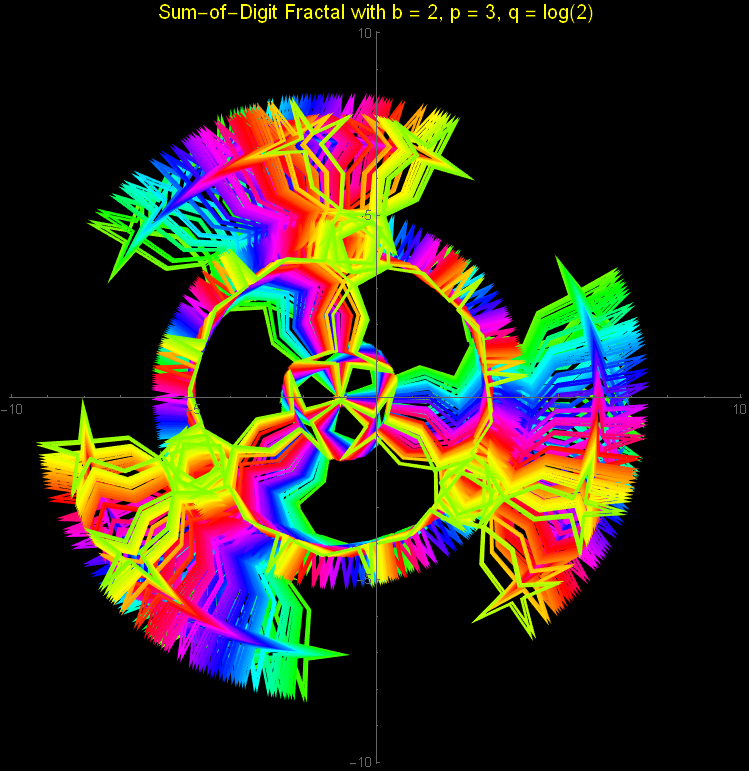
\includegraphics[width=0.48\textwidth,
    height=0.45\textwidth]{n(10000)_b(2)_p(3)_q(ln2).png}
    \end{center}
\vill
\end{multicols}
}

\headerbox{References}{column=1,span=1,below=fractalexamples}{
\begin{itemize}[leftmargin=0.15in]\compresslist
\item Dekking, F. Michel (1982). "On the distribution of digits in arithmetic sequences". \textit{Séminaire de théorie des nombres de Bordeaux}, 1-12.
\item Dekking, F.M., and Mendès France, M. (1981). "Uniform distribution modulo one: a geometrical viewpoint". \textit{Journal für die reine und angewandte Mathematik 329},  143-153.
\item 
Lehmer, D. H., and Emma Lehmer (1979). "Picturesque Exponential Sums, I". \textit{The American Mathematical Monthly 86.9}, 725-733.
\end{itemize}
}


\end{poster}
\end{document}